\documentclass[a4paper, 12pt]{article}
\usepackage[utf8]{inputenc}
\usepackage[slovak]{babel}
\usepackage{graphicx}
\usepackage{amsmath,amssymb,amsfonts}

\newenvironment{task}{}{}
\newenvironment{solution}{\noindent\textbf{Riešenie:}}{}


\begin{document}


\section*{B34A5A}
\begin{task}
    Nájdite prenosovú funkciu $F(s)=\dfrac{Y(s)}{W(s)}$ pre systém opísaný blokovou schémou: 

    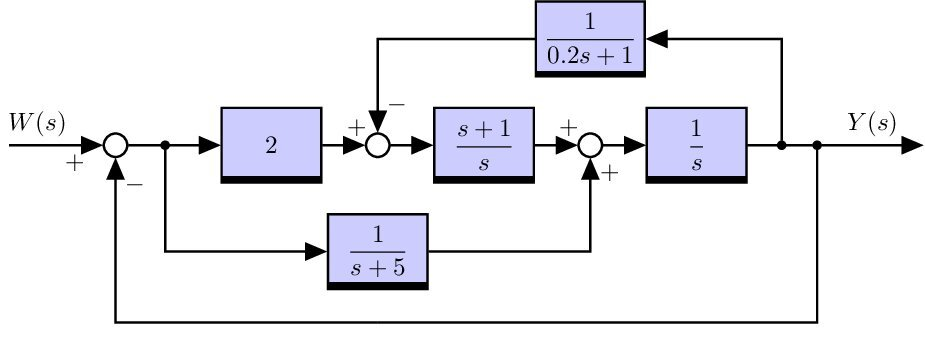
\includegraphics{../images/blokovka01_00002.jpg}
\end{task} 

\begin{solution}
    \begin{equation*}
        \dfrac{2s^2+13s+10}{s^3+7s^2+18s+15}
    \end{equation*}
\end{solution}

\section*{BA23B4}
\begin{task}
    Nájdite prenosovú funkciu $F(s)=\dfrac{Y(s)}{W(s)}$ pre systém opísaný blokovou schémou: 

    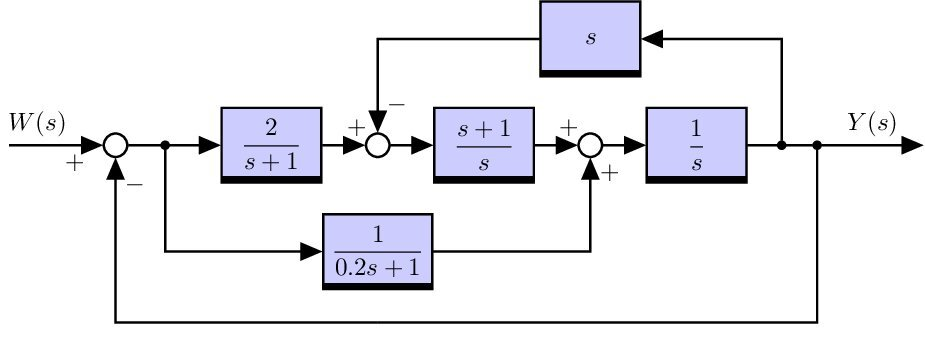
\includegraphics{../images/blokovka01_00003.jpg}
\end{task} 

\begin{solution}
    \begin{equation*}
        \dfrac{7s+10}{2s^3+11s^2+12s+10}
    \end{equation*}
\end{solution}

\section*{B2A76C}
\begin{task}
    Nájdite prenosovú funkciu $F(s)=\dfrac{Y(s)}{W(s)}$ pre systém opísaný blokovou schémou: 

    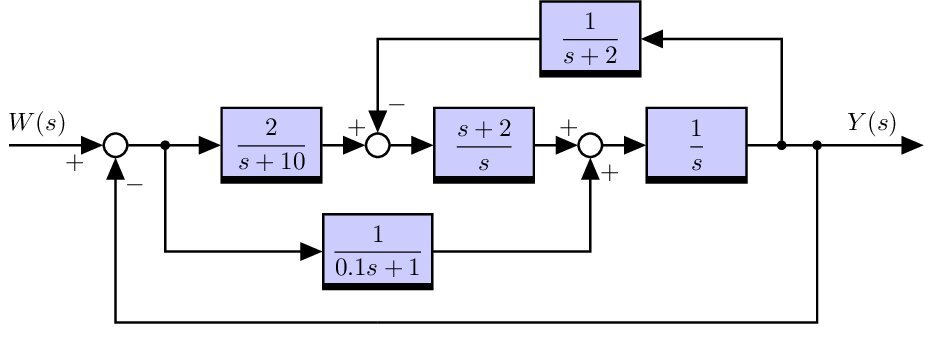
\includegraphics{../images/blokovka01_00004.jpg}
\end{task} 

\begin{solution}
    \begin{equation*}
        4\dfrac{3s+1}{s^3+10s^2+13s+14}
    \end{equation*}
\end{solution}


\end{document}
